% !TeX spellcheck = ru_RU
% !TeX program = xelatex
% !TeX encoding = UTF-8 Unicode

\documentclass{article}
\usepackage{xltxtra}
\usepackage{fontspec}
\usepackage{polyglossia}
% \usepackage{minted}
\setmainlanguage[babelshorthands=true]{russian}
\usepackage[usenames,dvipsnames,svgnames,table]{xcolor}
%\usepackage{calc}


% babel shorthands are:
%  "--- Cyrillic emdash in plain text.
%  "--~ Cyrillic emdash in compound names (surnames).
%  "--* Cyrillic emdash for denoting direct speech.
% "~ unbreakable hype. Example: как в 90"~х годах

\setotherlanguage{english}



\setmainfont{Cambria}
%\setromanfont{Times New Roman}
\setsansfont{Arial}
\setmonofont{Courier New}



% \newfontfamily{\cyrillicfontrm}{Times New Roman}
\newfontfamily{\cyrillicfonttt}{Courier New} 



\usepackage{graphicx}

\usepackage{wrapfig}
% !TeX root = rand_text.tex

\usepackage{xcolor}

\usepackage{tikz}
\usetikzlibrary{shapes,calc,positioning,graphs, arrows,patterns,through}


%\definecolor{gray50}{gray}{0.5}
\definecolor{myblue}{RGB}{12,131,200}
\definecolor{myred}{RGB}{200,100,100}
\definecolor{mydeepblue}{HTML}{1F2FAA}
    
%\tikzset{everypicture/.style=thick, rounded corners=5}
    


\tikzstyle{my lines} = [draw=blue!30,ultra thin]
\begin{document}

Коллекции на вкладке <<Вставка>> содержат элементы, которые определяют общий вид документа. Эти коллекции служат для вставки в документ таблиц, колонтитулов, списков, титульных страниц и других стандартных блоков. При создании рисунков, диаграмм или схем они согласовываются с видом текущего документа. Формат выделенного текста можно легко изменить, выбрав нужный вид из коллекции экспресс-стилей на вкладке ,,Главная``. Текст можно также отформатировать с помощью других элементов управления на вкладке <<Главная>>.



\tikzset{help lines/.style={color=blue!40,ultra thin} }

\begin{tikzpicture} 
	\draw [help lines] (0,0) grid (7,7) ;
\end{tikzpicture}

\tikzset{every node/.append style={font=\sffamily}}

\begin{tikzpicture}[help lines/.append style={step=5mm}]
    \draw [help lines] (0,0) grid (7,10) ;
    \filldraw[fill=gray!20, draw=black,very thick]  
        (1,1) rectangle node [fill=blue!10,draw=black,inner sep=10pt] {окно} +(5,5) 
        coordinate (ПравоВерх);
     \filldraw [fill=red!30] (ПравоВерх)   +(1,0) -- +(-2.5,2)  -- +(-6,0)  --cycle  ;
        
\end{tikzpicture}


Большинство элементов управления позволяют использовать вид из текущей темы и формат, указанный непосредственно. Чтобы изменить вид документа, выберите элементы темы на вкладке "Макет страницы". Состав коллекции экспресс-стилей можно изменить с помощью команды "Изменить текущий набор экспресс-стилей". Коллекции тем и экспресс-стилей включают команды восстановления, позволяющие вернуться к первоначальному виду документа, который содержится в текущем шаблоне. Коллекции на вкладке "Вставка" содержат элементы, которые определяют общий вид документа.

\begin{figure}[h]
\centering
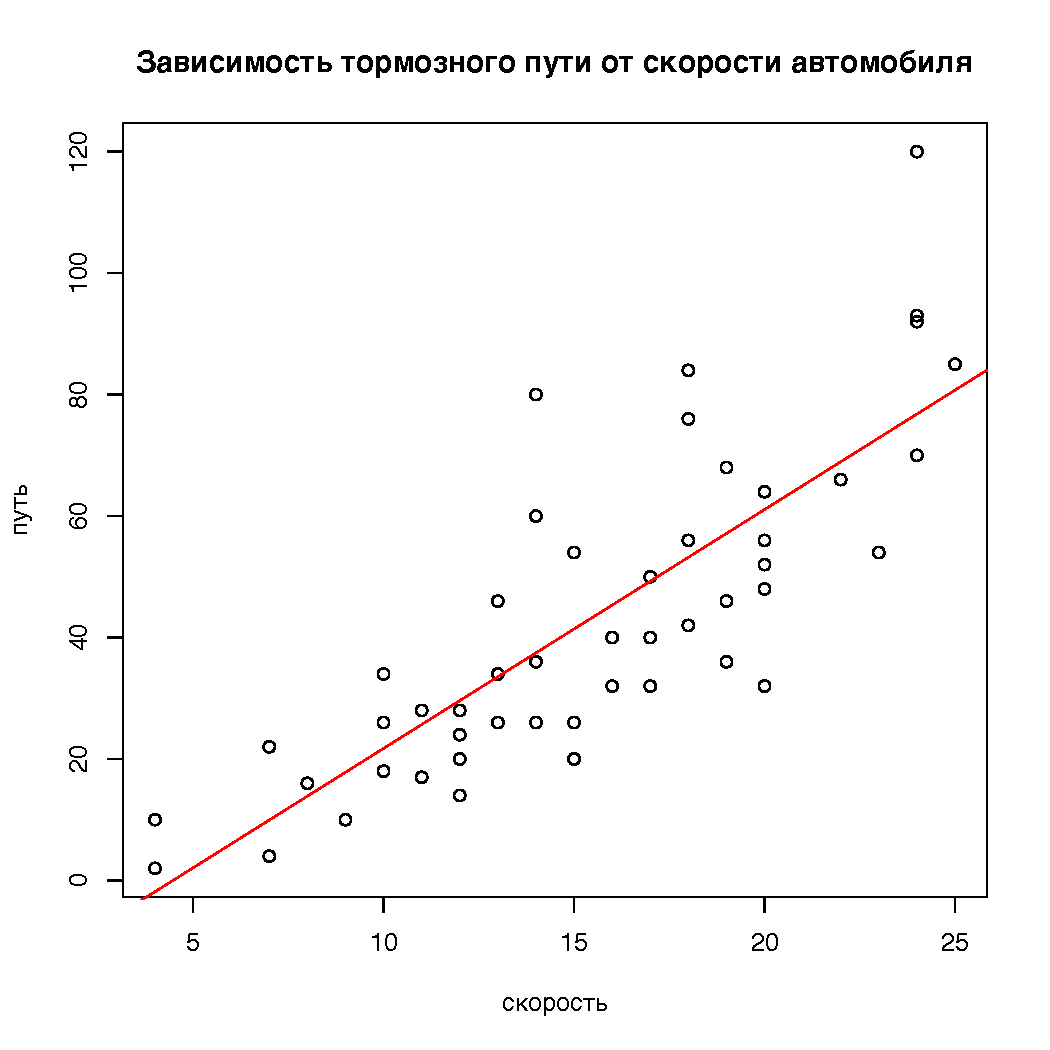
\includegraphics[height=10cm,width=0.5\textwidth,keepaspectratio,%
	trim=0 0.5cm 0 1.5cm,clip%
	]{plot_cars_distance}
\caption{График измерений тормозного пути}
\label{fig:plot_cars_distance}
\end{figure}


\begin{figure}[h]
    \centering
    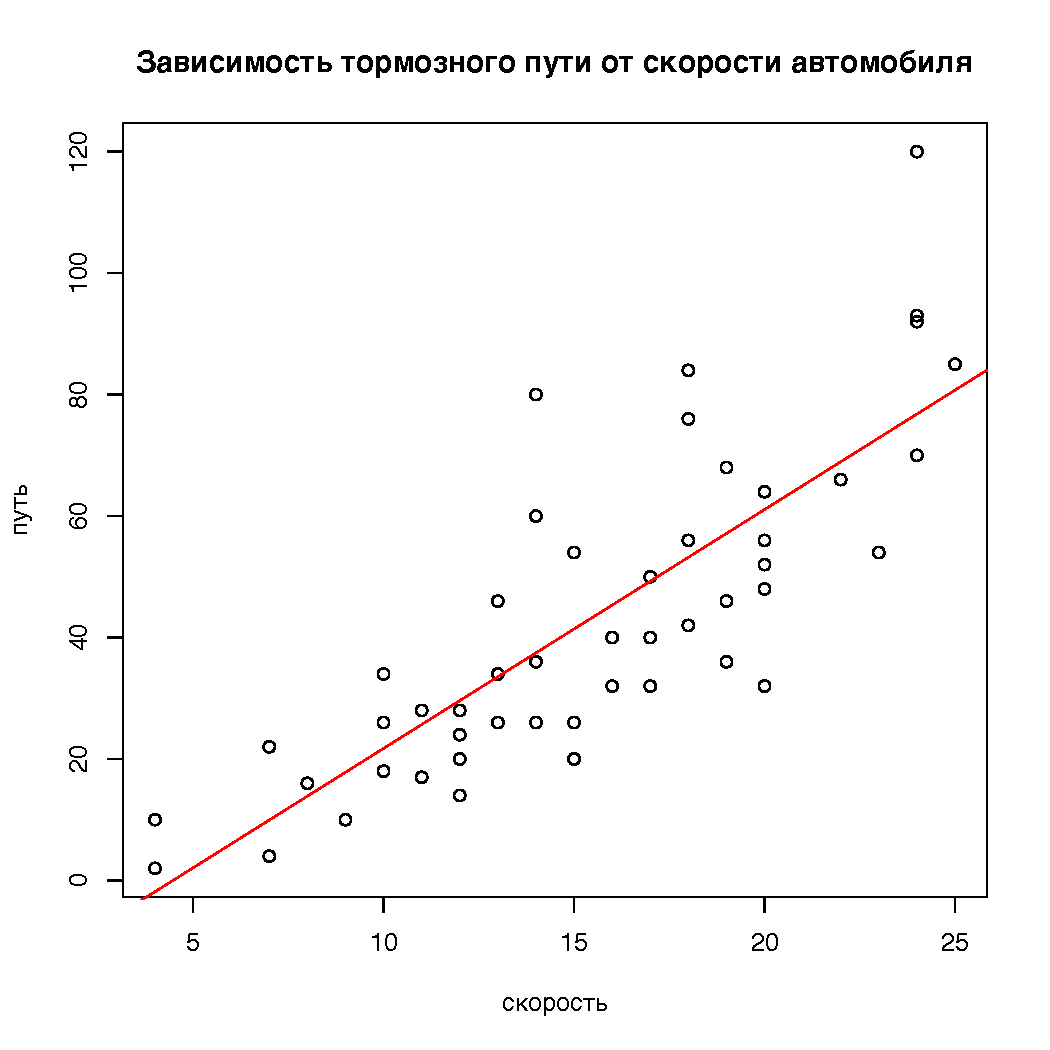
\includegraphics[height=10cm,width=0.5\textwidth,keepaspectratio,%
    trim=0 0.5cm 0 1.5cm,clip%
    ]{plot_cars_distance}
    
    
    {График измерений тормозного пути}
\end{figure}


Эти коллекции служат для вставки в документ таблиц, колонтитулов, списков, титульных страниц и других стандартных блоков. При создании рисунков, диаграмм или схем они согласовываются с видом текущего документа. Формат выделенного текста можно легко изменить, выбрав нужный вид из коллекции экспресс-стилей на вкладке "Главная". Текст можно также отформатировать с помощью других элементов управления на вкладке "Главная". Большинство элементов управления позволяют использовать вид из текущей темы и формат, указанный непосредственно.

\vspace{18pt}



Чтобы изменить вид документа, выберите элементы темы на вкладке "Макет страницы". Состав коллекции экспресс-стилей можно изменить с помощью команды "Изменить текущий набор экспресс-стилей". Коллекции тем и экспресс-стилей включают команды восстановления, позволяющие вернуться к первоначальному виду документа, который содержится в текущем шаблоне. Коллекции на вкладке "Вставка" содержат элементы, которые определяют общий вид документа. Эти коллекции служат для вставки в документ таблиц, колонтитулов, списков, титульных страниц и других стандартных блоков.
\begin{wrapfigure}{r}{0pt}
    
\includegraphics[width=0.4\linewidth]{tantau_129.jpg}
    \caption[Тантау]{Тиль Тантау - автор beamer и TikZ}
    \label{fig:4936_Tantau2}
\end{wrapfigure}

График зависимости см. на рис. \ref{fig:plot_cars_distance}

При создании рисунков, диаграмм или схем они согласовываются с видом текущего документа. Формат выделенного текста можно легко изменить, выбрав нужный вид из коллекции экспресс-стилей на вкладке "Главная". Текст можно также отформатировать с помощью других элементов управления на вкладке "Главная". Большинство элементов управления позволяют использовать вид из текущей темы и формат, указанный непосредственно. Чтобы изменить вид документа, выберите элементы темы на вкладке "Макет страницы".

\begin{figure}[h]
\centering	
% !TeX root = rand_text_14.tex

\tikzstyle{flownode} = [font=\sffamily,shape=rectangle,rounded corners=10pt, outer sep=1mm, minimum size=2cm,ultra thin,left color=gray!10,right color=cyan!60] 

%\tikzstyle{flowtext} = [sloped,yshift=2mm,font={\small\itshape}] ;

\tikzset{flowtext/.style = {sloped,below,font={\small\itshape} } } 

\begin{tikzpicture}[scale=0.6]
\node  (Банк) at (0,0) [flownode,right color=green!30] {Банк};
\node (Завод) [flownode,above = 3cm of Банк, draw]{Завод} ;
\node (Потребитель) [flownode,left =  2cm of Банк , draw]{Потребитель} ;


\draw [-stealth] (Банк)  edge 
     node  [flowtext] {деньги} 
         (Завод)
       (Потребитель)  edge 
            node  [flowtext]{деньги} 
                 (Банк) ;
\draw [stealth-,red]  (Потребитель)  edge 
node  [flowtext] {материальный поток} 
(Завод) ;
                 
\end{tikzpicture}


\caption{Потоки финансовые и материальные}
\end{figure}


Состав коллекции экспресс-стилей можно изменить с помощью команды "Изменить текущий набор экспресс-стилей". Коллекции тем и экспресс-стилей включают команды восстановления, позволяющие вернуться к первоначальному виду документа, который содержится в текущем шаблоне. Коллекции на вкладке "Вставка" содержат элементы, которые определяют общий вид документа. Эти коллекции служат для вставки в документ таблиц, колонтитулов, списков, титульных страниц и других стандартных блоков. При создании рисунков, диаграмм или схем они согласовываются с видом текущего документа.




Формат выделенного текста можно легко изменить, выбрав нужный вид из коллекции экспресс-стилей на вкладке "Главная". Текст можно также отформатировать с помощью других элементов управления на вкладке "Главная". Большинство элементов управления позволяют использовать вид из текущей темы и формат, указанный непосредственно. Чтобы изменить вид документа, выберите элементы темы на вкладке "Макет страницы". Состав коллекции экспресс-стилей можно изменить с помощью команды "Изменить текущий набор экспресс-стилей".



\end{document}

